\documentclass[tikz,border=5pt]{standalone}
\usepackage{pgfplots}
\pgfplotsset{compat=1.18}

\definecolor{corba}{HTML}{365FB3}
\definecolor{punt}{HTML}{B91C1C}
\definecolor{guia}{HTML}{6B7280}

\begin{document}
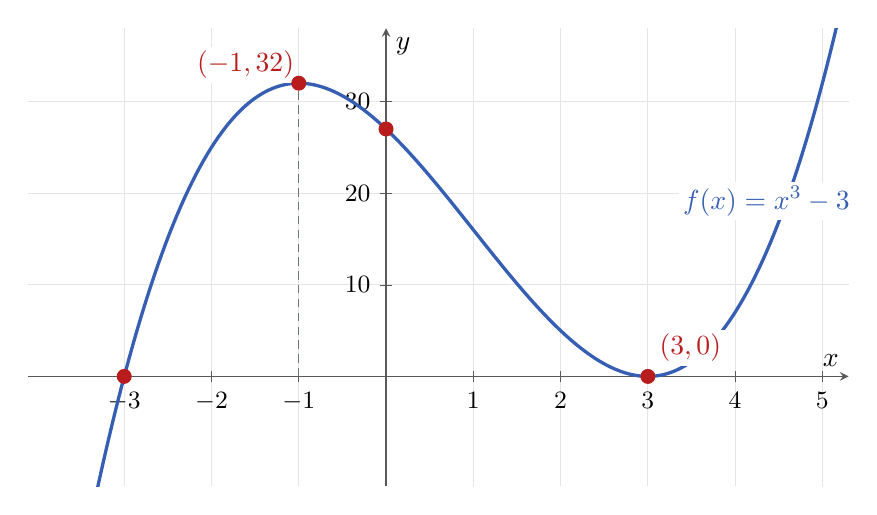
\begin{tikzpicture}
  \begin{axis}[
    width=12cm,
    height=7.4cm,
    axis lines=middle,
    xmin=-4.1,
    xmax=5.3,
    ymin=-12,
    ymax=38,
    xlabel={$x$},
    ylabel={$y$},
    xtick={-3,-2,-1,0,1,2,3,4,5},
    ytick={0,10,20,30},
    grid=major,
    grid style={black!10},
    axis line style={black!65},
    tick style={black!65},
    tick label style={font=\small},
    clip=true,
  ]
    \addplot[corba, very thick, domain=-4.05:5.25, samples=220]
      {x^3-3*x^2-9*x+27};
    \addplot[only marks, mark=*, mark size=2.5pt, punt]
      coordinates {(-3,0) (0,27) (-1,32) (3,0)};

    \draw[guia, densely dashed]
      (axis cs:-1,0) -- (axis cs:-1,32);
    \node[anchor=south east, text=punt, fill=white, inner sep=1.5pt]
      at (axis cs:-1,32) {$(-1,32)$};
    \node[anchor=south west, text=punt, fill=white, inner sep=1.5pt]
      at (axis cs:3.08,1.1) {$(3,0)$};
    \node[anchor=south west, text=corba, fill=white, inner sep=1.5pt]
      at (axis cs:3.35,17) {$f(x)=x^3-3x^2-9x+27$};
  \end{axis}
\end{tikzpicture}
\end{document}
